\documentclass[journal,10pt,twocolumn]{article}
\usepackage{graphicx, float}
\usepackage[margin=0.5in]{geometry}
\usepackage{amsmath, bm}
\usepackage{array}
\usepackage{booktabs}
\providecommand{\norm}[1]{\lVert#1\rVert}
\let\vec\mathbf
\newcommand{\myvec}[1]{\ensuremath{\begin{pmatrix}#1\end{pmatrix}}}
\newcommand{\mydet}[1]{\ensuremath{\begin{vmatrix}#1\end{vmatrix}}}

\title{\textbf{LINE}}
\author{VEMULAPALLI BAVYA SRI}
\date{October 2022}

\begin{document}

\maketitle
\paragraph{\textit{Problem Statement} -Let P=(-1, 0), Q = (0, 0) and R = (3, 3  $\sqrt{3}$  ) be three point. The equation of the bisector of the  $\angle(\vec{PQR})$ }
  
\section{Solution}

    Given  $\Vec{P}  =  \begin{pmatrix}
            -1\\ 
            0
            \end{pmatrix}$  ,
            $\vec{Q}  =  \begin{pmatrix}
            0 \\ 
            0
            \end{pmatrix}$
        and  $\vec{R}  =  \begin{pmatrix}
            3 \\ 
            -3\sqrt{3}
            \end{pmatrix}$
\begin{flushleft}
    Let  $\vec{M}$  be a point on the bisector.  $\vec{M}$  is equidistant from both the lines  $\vec{PQ}$ and   $\vec{QR}$ 
\vspace{0.1cm}

    
    Equation of the  $\vec{PQ}$  is given by
    
    \end{flushleft}
    
\begin{equation}
\vec{n_1}^\top \vec{x}= 0
\vspace{0.1cm}
\end{equation}
    
\begin{equation}
\vec{PQ} = \begin{pmatrix}
        1\\ 
        0
        \end{pmatrix} 
        \vspace{0.1cm}
\end{equation}
    
\begin{equation}
\vec{n_1}  =  \begin{pmatrix}
        0\\ 
        -1
        \end{pmatrix} 
        \vspace{0.1cm}
\end{equation}
    
\begin{equation}
\vec{n_1}^\top  =  \begin{pmatrix} 0  \ -1  \end{pmatrix} 
\vspace{0.1cm}
\end{equation}
    
\begin{equation}
\vec{n_1}^\top \vec{x}  =  \begin{pmatrix} 0  \ -1  \end{pmatrix}\vec{x} = 0 
\vspace{0.1cm}
\end{equation}
    
\begin{equation}
\lVert \vec{n_1}  \rVert = \sqrt{{\vec{n_1}}^\top \vec{n_1}}  
\vspace{0.1cm}
\end{equation}
    
\begin{equation}
=  \sqrt{(0)^2 + (-1)^2}   = 1
\vspace{0.1cm}
\end{equation}
    
\begin{flushleft}
    Equation of the  $\vec{QR}$  is given by
\end{flushleft}
    
\begin{equation}
\vec{n_2}^\top \vec{x} = 0 
\vspace{0.1cm}
\end{equation}
    
\begin{equation}
\vec{QR} = \begin{pmatrix}
        3\\ 
        3\sqrt{3}
        \end{pmatrix} 
        \vspace{0.1cm}
\end{equation}
    
\begin{equation}
\vec{n_2}  =  \begin{pmatrix}
        3\sqrt{3}\\ 
        -3
        \end{pmatrix} 
        \vspace{0.1cm}
\end{equation}
    
\begin{equation}
\vec{n_2}^\top  =  \begin{pmatrix} 3\sqrt{3}  \ -3  \end{pmatrix} 
\vspace{0.1cm}
\end{equation}
    
\begin{equation}
\vec{n_2}^\top \vec{x}  =  \begin{pmatrix} 3\sqrt{3}  \ -3  \end{pmatrix}\vec{x} = 0 
\vspace{0.1cm}
\end{equation}
    
\begin{equation}
\lVert \vec{n_2}  \rVert = \sqrt{{\vec{n_2}}^\top \vec{n_2}}  
\vspace{0.1cm}
\end{equation}
    
\begin{equation}
=  \sqrt{(3\sqrt{3})^2 + (-3)^2} = 6
\vspace{0.1cm}
\end{equation}
    
    As  $\vec{M}$  is equidistant from  $\vec{PQ}$  and  $\vec{QR}$ 
    
\begin{equation}
\frac{\lvert \mathbf{\vec{n_1}}^\top \vec{x} \rvert}{\lVert\vec{n_1} \rVert}  =  \frac{\lvert \mathbf{\vec{n_2}}^\top \vec{x} \rvert}{\lVert \vec{n_2} \rVert} 
\vspace{0.1cm}
\end{equation}
    
\begin{equation}
\frac{\begin{pmatrix} 0  \ -1  \end{pmatrix}\vec{x}}{1} = \frac{\begin{pmatrix} 3\sqrt{3}  \ -3 \end{pmatrix}\vec{x}}{6} 
\vspace{0.1cm}
\end{equation}
    
    By solving the above expression we get,
    \vspace{0.1cm}
    
\begin{equation}
    \begin{pmatrix} \sqrt{3}  \ 1\end{pmatrix}\vec{x} = 0
\end{equation}

\begin{equation}
    and \begin{pmatrix} \sqrt{3}  \ -1  \end{pmatrix}\vec{x} = 0
\end{equation}

\begin{flushleft}
    Equations (17) and (18) represent the equations of internal and external angular bisectors of  $\angle(\vec{PQR})$ .
    \vspace{0.1cm}
    
    Hence the required equation of the internal angular bisector of the  $\angle(\vec{PQR})$  is
    \end{flushleft}
    
\begin{table}[H]
    \begin{equation}
    \begin{tabular}{|l|c|c|c|c|c|c|c|c}\hline\textbf{ $\begin{pmatrix} \sqrt{3}  \ 1\end{pmatrix}\vec{x} = 0$}\\\hline
    \end{tabular}
    \end{equation}
\end{table}

\begin{flushleft}
    The generalised form of the above equation is given by 
\end{flushleft}
\begin{equation}
     \sqrt{3}x + y = 0 
\end{equation}
    
    
\section{Construction}

\begin{table}[h]
	\centering
\setlength\extrarowheight{2pt}
	\begin{tabular}{|c|c|c|}
		\hline
		\textbf{Symbol} & \textbf{Value} & \textbf{Description} \\
		\hline
		P & (-1,0) & point P\\
		\hline
		Q & (0,0) & point Q\\
		\hline
		R & (3$\sqrt{3}$,3) & point R\\
		\hline
		M & (-0.7,1.21) & point M\\
		\hline
	\end{tabular}
\end{table}

\begin{figure}[H]
    \centering
    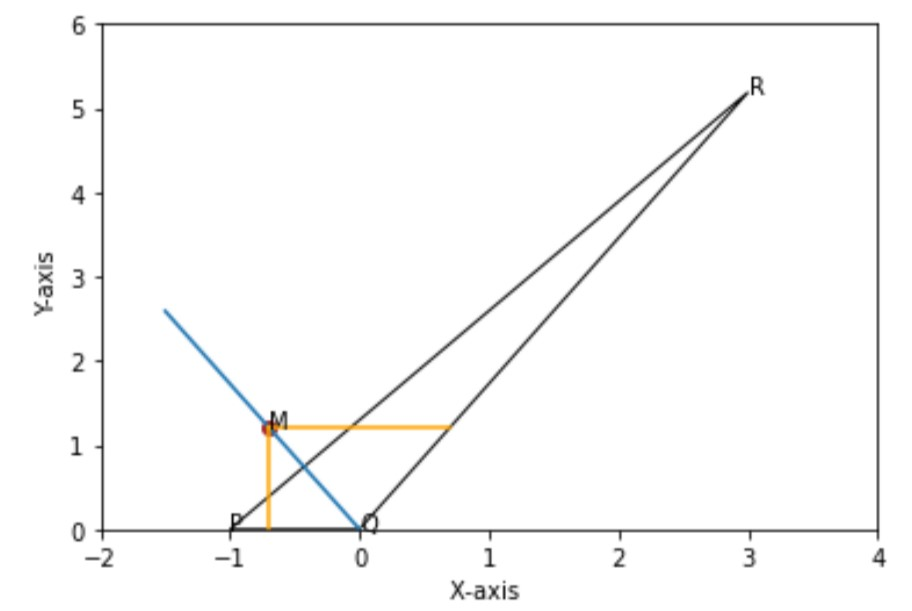
\includegraphics[scale=0.5]{diagram.jpg}
    \caption{Bisector}
    \label{fig:Bisector}
\end{figure}

    The above construction is realized by executing the following code.
    
\begin{table}[H]
\begin{tabular}{|l|c|c|c|c|c|c|c|c}\hline\textbf{https://raw.githubusercontent.com}\\
    \textbf{/BavyaVemulapalli/FWC-IITH/main/Line/Code/line.py} \\ \hline
\end{tabular}
\end{table}

\section{Conclusion}

    Hence, the equation of the bisector of angle PQR was found using matrices.

\end{document}